\subsection{Esercizio 21}
Costruire una tabella in cui viene riportato, al crescere di $n$, il massimo errore di
interpolazione ottenuto approssimando la funzione:
\[
    f(x) = \frac{1}{2(2x^2-2x+1)}
\]
sulle ascisse $x_0 \le x_1 \dots \le x_n$:
\begin{itemize}
    \item equidistanti in $[-2, 3]$,
    \item di Chebyshev per lo stesso intervallo,
\end{itemize}
utilizzando le function degli Esercizi 16-18 e 20, e la function $spline$ di Matlab. Considerare
$n = 4, 8, 16, \dots, 40$ e stimare l'errore di interpolazione su 10001 punti
equidistanti nell'intervallo $[x0, xn]$.
\newline \textbf{Soluzione:}

Eseguendo lo script \nameref{cod:21} si ottengono i risultati contenuti nella
tabella \ref{tab:21_equidistant} e nella figura \ref{fig:es21_equidistant} per
i valori equidistanti, e nella tabella \ref{tab:21_chebyshev} con figura
\ref{fig:es21_chebyshev} per i punti di Chebyshev. Le figure rappresentano
il logaritmo naturale di errore di interpolazione data eccessiva differenza tra
alcuni valori.
\begin{figure}[!ht]
    \centering
    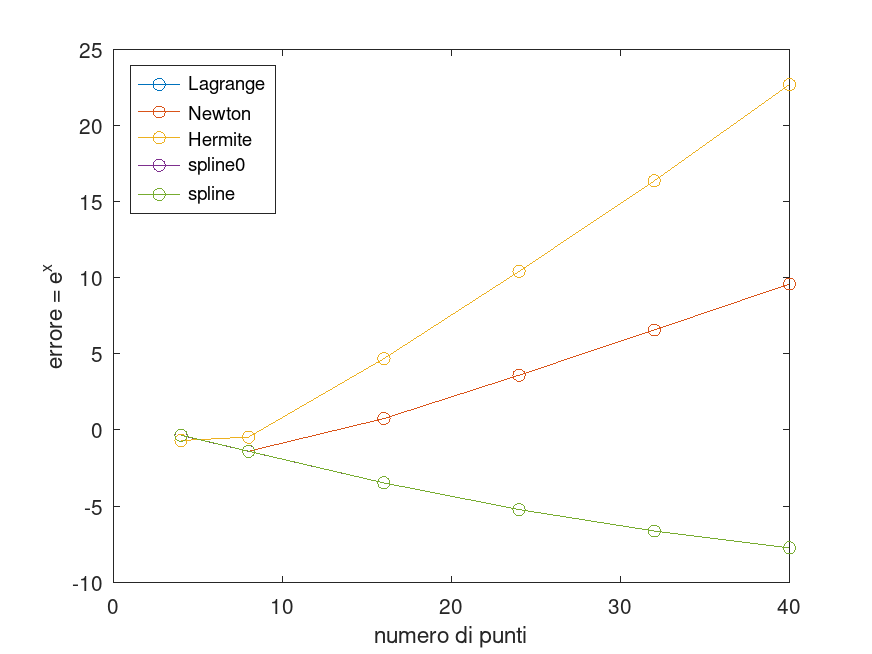
\includegraphics[width=16cm,height=10cm,keepaspectratio]{capitolo5/es21_figure_equidistant.png}
    \caption{logaritmo di errore per punti equidistanti}
    \label{fig:es21_equidistant}
\end{figure}
\FloatBarrier
\begin{table}[ht]
    \centering
    \renewcommand\arraystretch{2}
    \resizebox{\columnwidth}{!}{
        \begin{tabular}{| l l l l l l l|}
            \hline
            Punti equidistanti & \vline & Lagrange              & Newton                & Hermite               & spline0               & spline                \\
            \hline
            4                  & \vline & 7.070135746606334e-01 & 7.070135746606335e-01 & 4.998681947544072e-01 & 7.013574660633484e-01 & 7.070135746606334e-01 \\
            8                  & \vline & 2.473586065593151e-01 & 2.473586065593149e-01 & 6.264604673549260e-01 & 2.460753323436625e-01 & 2.471061445541360e-01 \\
            16                 & \vline & 2.107551869554541e+00 & 2.107551869554544e+00 & 1.075622144776140e+02 & 3.089074684813331e-02 & 3.089073253328134e-02 \\
            32                 & \vline & 7.052964658239763e+02 & 7.052964659260714e+02 & 1.258745533449631e+07 & 1.314616578641292e-03 & 1.314616578444783e-03 \\
            40                 & \vline & 1.446715032523167e+04 & 1.446715059723064e+04 & 6.999722473595546e+09 & 4.338554349913037e-04 & 4.338554349905266e-04 \\
            \hline
        \end{tabular}
    }
    \caption{valori approssimati usando metodi di Lagrange, Newton, Hermite, spline0 e spline}
    \label{tab:21_equidistant}
\end{table}
\begin{figure}[!ht]
    \centering
    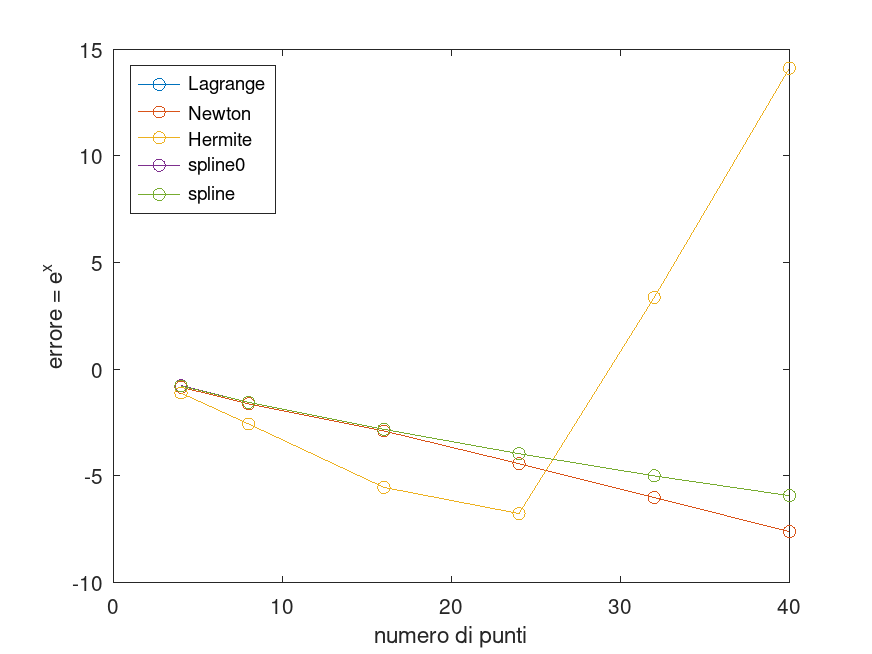
\includegraphics[width=16cm,height=10cm,keepaspectratio]{capitolo5/es21_figure_chebyshev.png}
    \caption{logaritmo di errore per punti di Chebyshev}
    \label{fig:es21_chebyshev}
\end{figure}
\FloatBarrier
\begin{table}[ht]
    \centering
    \renewcommand\arraystretch{2}
    \resizebox{\columnwidth}{!}{
        \begin{tabular}{| l l l l l l l|}
            \hline
            Punti Chebyshev & \vline & Lagrange              & Newton                & Hermite               & spline0               & spline                \\
            \hline
            4               & \vline & 4.260576750985503e-01 & 4.260576750985503e-01 & 3.240683104948798e-01 & 4.590450881560625e-01 & 4.504797289451788e-01 \\
            8               & \vline & 1.953973472974986e-01 & 1.953973472974987e-01 & 7.594297302032840e-02 & 2.098328475015154e-01 & 2.098569436714917e-01 \\
            16              & \vline & 5.474819091789429e-02 & 5.474819091789429e-02 & 3.890209538672640e-03 & 5.908465722169787e-02 & 5.908464936973012e-02 \\
            32              & \vline & 2.418340324994994e-03 & 2.418340324994994e-03 & 2.864094265641310e+01 & 6.658092179819830e-03 & 6.658092179763764e-03 \\
            40              & \vline & 4.874049664271851e-04 & 4.874049664275182e-04 & 1.339175914816082e+06 & 2.636728138104893e-03 & 2.636728138104671e-03 \\
            \hline
        \end{tabular}
    }
    \caption{valori approssimati usando metodi di Lagrange, Newton, Hermite, spline0 e spline}
    \label{tab:21_chebyshev}
\end{table}

